% ------ PREAMBLE ------ 
\documentclass[10pt,a4paper,twocolumn]{article}
\usepackage[utf8]{inputenc}
\usepackage[english, french]{babel}
\usepackage[margin=2cm]{geometry}
\renewcommand{\baselinestretch}{1.05} 

\usepackage{sansmathfonts}
\usepackage{fontspec}
\setmainfont{Latin Modern Sans}

\usepackage{physics}
\usepackage[shortlabels]{enumitem}
\usepackage{algpseudocode}
\usepackage{algorithm}
\AtBeginDocument{\RenewCommandCopy\qty\SI}
\usepackage{amsmath,amsfonts,amssymb}
\newcommand\inlineeqno{\stepcounter{equation}\ (\theequation)}
\usepackage{derivative}
\DeclareDifferential{\dd}{\mathrm{d}}
\usepackage{graphicx}
\graphicspath{{images/}}
\usepackage{subfig}
\usepackage{float}
\usepackage{caption}
\captionsetup{font={small, color={Gray2}}, labelfont={sf, bf}, textfont={sf,sansmath}, labelsep=colon}
\usepackage{siunitx}
\sisetup{detect-all,
	separate-uncertainty = true,
	uncertainty-separator = {\,\pm\,},
	multi-part-units=single
}
\DeclareSIUnit{\year}{yr}
\usepackage[dvipsnames]{xcolor}
\definecolor{Gray1}{RGB}{101, 101, 101}
\definecolor{Gray2}{RGB}{60, 60, 60}
\definecolor{Code}{RGB}{230, 235, 255}

% useful commands for typing ML 
\newcommand{\bs}[1]{\boldsymbol{#1}}
\newcommand{\mb}[1]{\mathbold{#1}}
\newcommand{\T}{^{\intercal}}
\newcommand{\R}[1]{\mathbb{R}^{#1}}
\newcommand{\C}{\mathcal{C}}
\newcommand{\curr}{^{\langle t \rangle}}
\newcommand{\prev}{^{\langle t-1 \rangle}}
\newcommand{\sk}{\texttt{scikit-learn}}
\newcommand{\tf}{\texttt{tensorflow}}
\newcommand{\py}[1]{\texttt{#1}}
\newcommand{\ie}{\emph{i.e.} }
\newcommand{\pjone}{\href{https://github.com/p-perrone/UiO_MachineLearning/blob/main/ml_project1/latex/Perrone_MLProject1.pdf}{report from Project 1}}
\newcommand{\pjtwo}{\href{https://github.com/p-perrone/UiO_MachineLearning/blob/main/ml_project2/latex/Perrone_MLProject2.pdf}{report from Project 2}}


\usepackage[most]{tcolorbox}
\tcbset{on line, 
	boxsep=4pt, left=0pt,right=0pt,top=0pt,bottom=0pt,
	colframe=white,colback=Code,  
	highlight math style={enhanced}
}
\let\oldtexttt\texttt
\renewcommand{\texttt}[1]{\tcbox[boxsep=1pt, left=2pt, right=2pt]{\oldtexttt{#1}}}

\tcbuselibrary{theorems}
\newtcbtheorem[number within=section]{mytheo}{Theorem}%
{colback=blue!3,colframe=blue!35!white,fonttitle=\bfseries}{th}

\usepackage[colorlinks=true, 
linkcolor=Plum, 
citecolor=RoyalBlue, 
urlcolor=BlueViolet]{hyperref}
\usepackage{booktabs}
\usepackage{multirow}
\usepackage{setspace}
\usepackage{pdfpages}
\usepackage{pythonhighlight}
\usepackage{verbatim}
\usepackage{fancyhdr}
\usepackage{lipsum}
\pagestyle{fancy}
\fancyhf{} 
\fancyhead[L]{\leftmark}
\fancyfoot[C]{\thepage} 

\title{
	\bfseries PROJECT 3: \\
	
	Forecasting short-term evolution of snow pack thickness with recurrent neural networks (RNNs): an application of Long-Short Term Memory (LSTM) algorithm\\
	\vspace{1cm}
	\large
	Applied Data Analysis and Machine Learning\\
	FYS-STK4155 - University of Oslo
}
\author{
	\textbf{Pietro PERRONE}\\
	\href{mailto:pietrope@uio.no}{pietrope@uio.no}
} 
\date{November 20, 2025}

% Section formatting
\usepackage{titlesec}
\titleformat{\section}
{\color{RoyalBlue}\titlerule[1.5pt]\LARGE\fontseries{sbc}\sffamily\selectfont\color{RoyalBlue}}
{\thesection}
{1em}
{}
\titleformat{\subsection}
{\Large\fontseries{sbc}\selectfont\sffamily\color{Gray2}}
{\thesubsection}
{1em}
{}
\titleformat{\subsubsection}
{\large\fontseries{sbc}\slshape\sffamily\color{Gray2}}
{\thesubsection.\alph{subsubsection}}
{1em}
{}
\titleformat{\paragraph}
{\normalfont\fontseries{sbc}\slshape\sffamily\color{Gray2}}
{\theparagraph}
{0.5em}
{}

\usepackage[backend=biber, style=apa]{biblatex}
\addbibresource{project3.bib}

% ------ DOCUMENT ------ 

\begin{document}
	\selectlanguage{english}
	
	\begin{titlepage}
		
		\begin{figure}
			\centering
			\includegraphics[width=0.7\textwidth]{uio.pdf}
		\end{figure}
		
		\maketitle
		
		\centering
		
		
		\textbf{GitHub link to the project repository:\\
			\url{https://github.com/p-perrone/UiO_MachineLearning/tree/main/ml_project3}}
		
		\textbf{Link to DeepSeek chat:\\
			\url{https://chat.deepseek.com/share/i38u41hr9ln9ruwnxh}}
		
		\vspace{2cm}
		
		\begin{abstract}
		
		\end{abstract}
		
	\end{titlepage}
	\onecolumn
	
	\tableofcontents
	
	\twocolumn
	
\section{Introduction}
Snowpack plays a key role in mountain hydrology and climate systems, acting as a natural reservoir that stores precipitation in winter and releases it during melt periods, thereby controlling streamflow, water availability, and flood risk \parencite{derySnowClimatePhysical2010, dewallePrinciplesSnowHydrology2008, dengGlacierSnowVariations2019}. As a seasonal component of the cryosphere, it contributes to the regulation of global surface energy balance, reflecting solar radiation thanks to its bright surface, low in absorptivity and transmissivity \parencite{roeschEvaluationSurfaceAlbedo2006, maleSnowSurfaceEnergy1981}. Its evolution is governed by energy and mass balance processes, primarily snowfall, compaction, metamorphism, melt, and sublimation, which are strongly influenced by meteorological variables such as temperature, precipitation, solar radiation, cloud cover, humidity, and wind. 

Accurate snowpack forecasting is therefore crucial for water resource management, hydropower production, avalanche forecasting, and climate impact studies. Methods range from physically based snow models that explicitly solve energy and mass balance equations, to statistical and data-driven approaches that exploit empirical relationships between snow variables and meteorological forcings \parencite{karevanTransductiveLSTMTimeseries2020, picardSimulationSnowAlbedo2024, gustafssonSurfaceEnergyBalance2001, houImpactsSnowChanges2025, houImpactsSnowChanges2025,magnussonImprovingHydropowerInflow2020}. In recent years, hybrid and machine-learning approaches, including regularized regression and sequence-based models, have gained traction for short-term snowpack prediction, particularly in contexts where dense observations are available and computational efficiency is required. Many of these studies implement Recurrent Neural Networks (RNNs), especially Long Short-Term Memory (LSTM) architectures, which are well suited for time-series modeling \parencite{blandiniLearningFilterSnow2025, wangExploringPotentialLong2022}. 

RNNs are a class of neural architectures specifically designed to model sequential data by explicitly accounting for temporal dependencies through recurrent connections. However, standard RNNs suffer from vanishing and exploding gradient problems, which limit their ability to learn long-term dependencies. Long Short-Term Memory (LSTM) networks address these limitations by introducing a gated memory cell that regulate information flow, allowing the network to retain and update relevant informations over a given time horizon \parencite{hochreiters.LongShortTermMemory1997, gravesSupervisedSequenceLabelling2012, hewageLongshortTermMemory2019}. As a result, LSTMs have become a standard choice for time-series prediction in geosciences and hydrology, including snow and meteorological applications Compared to physically based models, the advantages of such methods depend on the specific objective and include: (i) robustness in capturing complex, non-linear relationships among meteorological variables without the need for explicit physical approximations, (ii) effective performance under limited observational availability, such as sparse weather stations or missing snow profile data, and (iii) relatively low computational cost, particularly once trained \parencite{hewageLongshortTermMemory2019, kumarComparativeAnalysisVarious2025}. 

Given the fairly recent diffusion of such techniques in geosciences contexts, it is crucial to properly understand their behavior and efficiency. In particular, for meteorological forecasting it is important to identify which variables play a dominant role in the model and to assess the required level of complexity, since over-parameterization may lead to unnecessary computational cost and reduced interpretability. In this study, we address these issues by performing an explicit selection of the input parameters (\emph{i.e.}, the features) and by testing the forecasting capabilities of a sequential model based on Long Short-Term Memory (LSTM) networks, implemented using the \texttt{TensorFlow} Python module \parencite{tensorflow_sequential}. Hourly meteorological data provided by the \href{https://cf.regione.vda.it/en/the-aosta-valley-functional-center}{Functional Centre} of the Aosta Valley Region (Western Alps, Italy) are used to predict the short-term evolution (24 hours) of snowpack at a weather station located at \qty{1960}{\meter} a.s.l.. Such data are available on the Centre's website, and are very representative of typical mountain weather stations; for these reasons, we chose them for this analyis.
The analysis is structured as follows:
\begin{enumerate}[(a)]
	\item \textbf{Preprocessing}: loading 35~days of data (November–December 2025) from the Functional Centre, followed by scaling and gap filling (handling of missing values);
	\item \textbf{Feature selection}: splitting the dataset into training and testing subsets; fitting linear models with Ridge and Lasso (L2 and L1) regularization; tuning through bootstrapping, and evaluating coefficient stability and Mean Squared Error to assess the relative importance of each meteorological variable;
	\item \textbf{LSTM forecasting}: chronological splitting of the dataset into training and forecasting periods; construction of input sequences; evaluation of forecasting performance under different model complexities and feature sets (\ie tuning of hyperparameters); forecasting and computational time estimation through bootstrapping.
\end{enumerate}

\section{Materials and methods}
\begin{figure}[t]
	\centering
	\includegraphics[width=\columnwidth]{timeseries.pdf}
	\caption{\textbf{Time series of meteorological variables} | The diurnal-nocturnal cyclic patterns can be observed in solar radiation and temperature}
	\label{fig:ts}
\end{figure}

\subsection{Data}
The weather measurements we employed were collected at Pont Valsavarenche (\url{https://presidi2.regione.vda.it/str_dataview_station/3070}). The weather station is located at \qty{1951}{\metre} a.s.l. on the bottom of glacial valley (45.5268 °N, 7.20093 °E in Coordinate Reference System WGS84 - EPSG:4326), it is equipped a mechanical pluviometre, an anemometer, and regular weather stations instrumentation. They are hourly based, and are summarized in Table \ref{tab:variables}; a 10 days time series is also shown in Figure \ref{fig:ts}, to give an overarching view of typical patterns followed by such variables. Each parameters corresponds to one of the features that our models will employ to forecast either snow depth and temperature. They range from November 2 to December 5 2025.
\begin{table*}[h]
	\centering
	\caption{Meteorological variables used in the analysis.}
	\label{tab:variables}
	\begin{tabular}{lSl}
		\toprule
		\textbf{Variable} & {\textbf{Unit}} & \textbf{Description} \\
		\midrule
		Snow depth            & \unit{\centi\metre}              & Total snowpack depth measured at the station \\
		Irradiation           & \unit{\watt\per\metre\squared}   & Incoming shortwave solar radiation at the surface \\
		Precipitation         & \unit{\milli\metre}              & Liquid-equivalent precipitation amount \\
		Relative humidity     & \unit{\percent}                  & Ratio of actual to saturation water vapour content \\
		Wind speed            & \unit{\metre\per\second}         & Horizontal wind velocity at measurement height \\
		Air temperature       & \unit{\degreeCelsius}            & Near-surface air temperature \\
		\bottomrule
	\end{tabular}
\end{table*}

\subsection{Theory of central algorithms}
In the following sections, we address all the different variables with specific symbology. The training design matrix $\bs{X}$ is composed of $n = \sim720$ samples ($30\,\text{days} \times 24\,\text{hours}$)  and a variable amount of features $p$ (2 to 6, depending on the model), that represent the different meteorological variables. $\bs{y}$ is the true (observed) set of values, typically 24 in total, that the models aim to reproduce, by minimizing the loss between this last and the forecasted values $\bs{\tilde{y}}$. The set of optimal parameters obtained through such minimization is denoted $\bs{\theta}$, hence $\bs{\tilde{y}} = \bs{X\theta}$.

	\subsubsection{Scaling the data}
We applied standard scaling to all the input data. Given an a vector $\bs{x}$, all its elements are subtracted by its mean and divided by its standard deviation \parencite{hastie2009elements}:
\begin{equation}
	x_i \rightarrow \frac{x_i - \overline{x}}{\sigma(\boldsymbol{x})}
\end{equation}
Standard scaling has been chosen over other scaling methods, since our former dataset does not show any strong outliers, and it has been previously found that this technique yields highest level of accuracy in geoscientific contexts \parencite{katipogluImpactPreprocessingApproaches2023, nishatInvestigatingApplicabilityLong2025, poushiExploringMachineLearning}.


	\subsubsection{Feature selection: bootstrapping with Ridge and Lasso regularizations}
Feature selection was performed by computing the optimal values of each parameter with Ridge and Lasso linear models. These analysis methods modify the simplest form of ordinary least squares (OLS), by adding a penalty to the cost function $\mathcal{C}(\bs{y, X, \theta})$ that results in a shrinkage of optimal parameters. 

Ridge applies an L2-regularization, \ie adds an L2-norm $\norm{\bs{\theta}}_2$, minimizing as follows:
\begin{equation}
	{\displaystyle \min_{\boldsymbol{\theta}\in
			{\mathbb{R}}^{p}}} \left[\mathcal{C}(\bs{y, X, \theta})+\lambda\vert\vert \boldsymbol{\theta}\vert\vert_2^2\right]
\end{equation}
Lasso adds an L1-norm $\norm{\bs{\theta}}_1$:
\begin{equation}
	{\displaystyle \min_{\boldsymbol{\theta}\in
			{\mathbb{R}}^{p}}}\left[\mathcal{C}(\bs{y, X, \theta})+\lambda\vert\vert \boldsymbol{\theta}\vert\vert_1\right]
\end{equation}
The L2-norm is given by the sum of squares of all the optimal parameters, whereas the L1-norm by the sum of the absolute values \parencite{hastie2009elements}. More informations are also available in \href{https://github.com/p-perrone/UiO_MachineLearning/blob/main/ml_project1/latex/Perrone_MLProject1.pdf}{report from Project 1}. For the aim of this work, it is relevant to underline the different behaviors of such methods in feature selection: Ridge, by adding a squared norm, never shrinks the parameters to 0, whereas Lasso does. Ridge is therefore useful for assessing relative feature importance, but Lasso has to be used to actually select only the features to retain \parencite{tibshiraniRegressionShrinkageSelection1996}.

All the regressors that we implemented in this work minimize the same cost function, the \emph{Mean Squared Error} MSE:
\begin{equation}
	\mathcal{C}(\bs{y}, \bs{\tilde{y}}) : \mathrm{MSE}(\boldsymbol{y},\boldsymbol{\tilde{y}}) = \frac{1}{n}
	\sum_{i=0}^{n-1}(y_i-\tilde{y}_i)^2
\end{equation}
\href{https://github.com/p-perrone/UiO_MachineLearning/blob/main/ml_project1/latex/Perrone_MLProject1.pdf}{Report from Project 1} contains further informations on this function. It represents a standard in minimization problems, notably in geosciences contexts \parencite{guptaDecompositionMeanSquared2009, linesReviewLeastsquaresInversion1984}. Its quadratic form ensures smooth and twice-differentiable gradients, enabling efficient optimization with gradient-based methods, and leads to a convex objective function in linear models with a unique global minimum \parencite{bishop2006_pattern, hastie2009elements}. Moreover, minimizing MSE corresponds to maximum likelihood estimation under the assumption of Gaussian-distributed errors, providing a clear probabilistic interpretation \parencite{wassermanLinearLogisticRegression2004}.

Bootstrapping (more insights in \pjone) provides an empirical distribution of parameters estimates by repeatedly
resampling the training set with replacement and refitting the model for a number of bootstraps $B$. We employed this resampling method for evaluating the loss and the stability of each feature coefficient resulting from Ridge and Lasso refitting.
We chose MSE as loss function and sign--stability as metrics. Sign stability is a feature-selection criterion that assesses whether the direction (sign) of a regression coefficient is consistent under resampling. Let $\bs{\theta}$ the optimal parameters vector fitted on the full dataset, and $\bs{\theta}^{*(b)}$ the estimate from bootstrap replicate $b$.
For each feature $j$, the sign--stability score is defined as
\begin{equation}
S_j = \frac{1}{B} \sum_{b=1}^B  \!\left[\,\mathrm{sign}\!\left(\theta^{*(b)}_j\right)
= \mathrm{sign}\!\left(\theta_j\right)\right],
\end{equation}
which measures how consistently a feature keeps the same directional effect.
Features with high stability (e.g., $S_j \approx 1$) are considered reliable,
while unstable features are likely noise \parencite{zouRegularizationVariableSelection2005, meinshausen2010stability}.
Once computed MSE and sign--stability for each parameter, the final selection is carried out by setting a minimal threshold based on the maximum value of the optimal parameters vector, base on \cite{kumarComparativeAnalysisVarious2025}; each $j$-th parameter is selected only if its absolute value is greater than this threshold:
\begin{equation} \label{eq:tsc}
	\abs{\theta_j} \geq k \abs{\max(\bs{\theta})}
\end{equation}
with $k = 0.01$, denoting a significance level factor.

	\subsubsection{RNNs and Long Short-Term Memory}
\begin{figure*}[t]
	\centering
	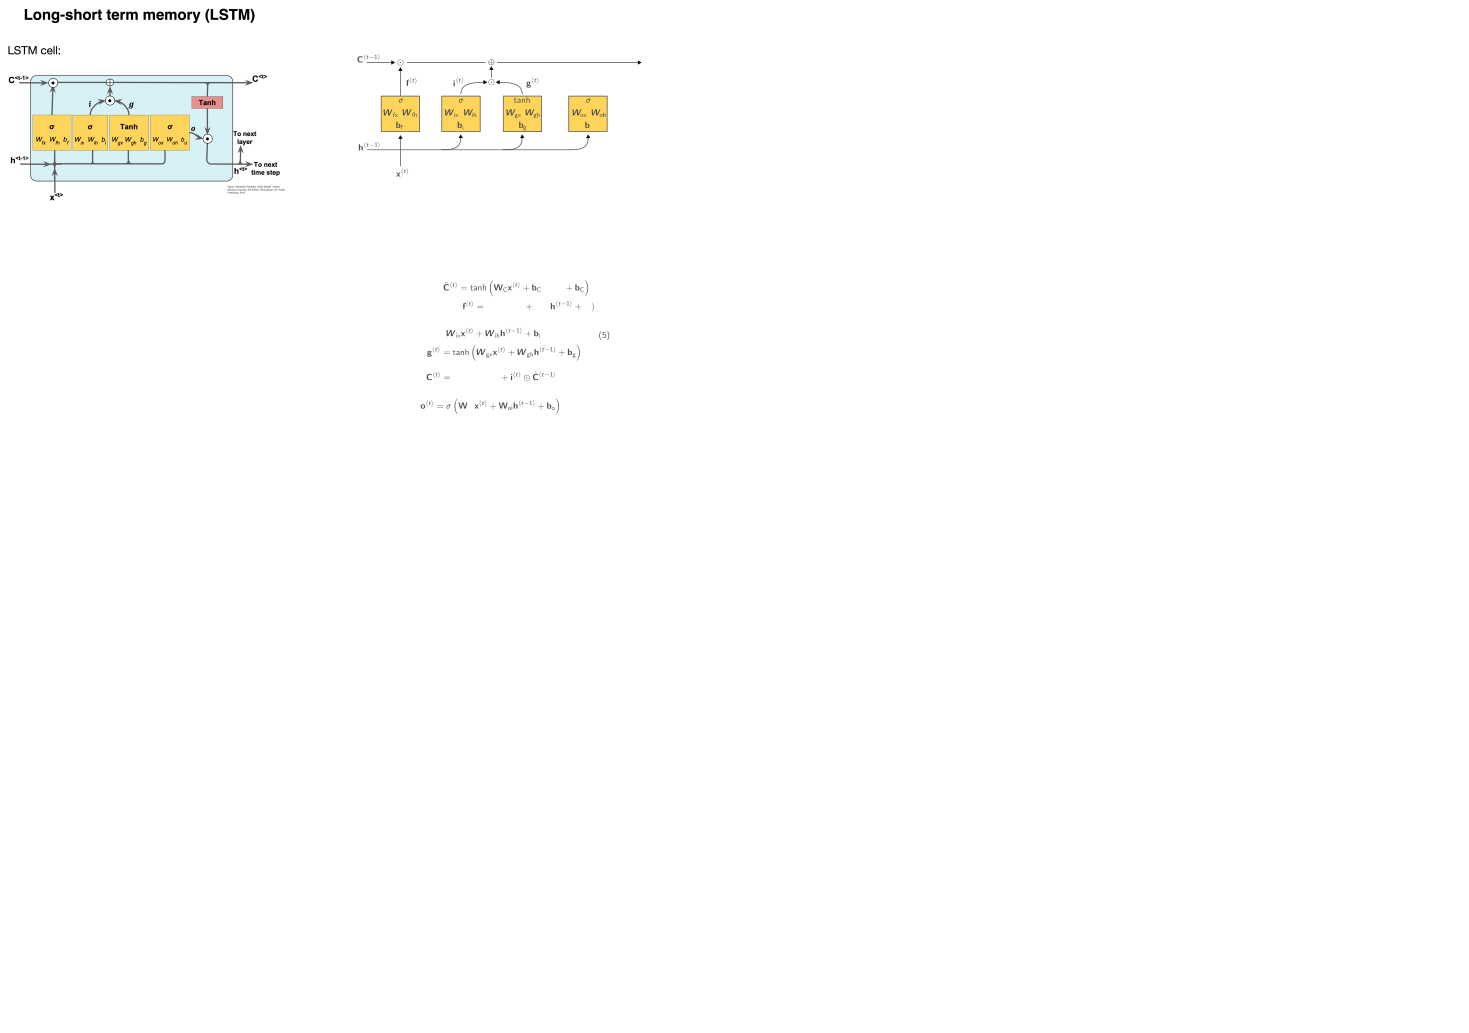
\includegraphics[width=\textwidth]{LSTM.pdf}
	\caption{\textbf{Long Short-Term Memory unit} | LSTM is characterized by a hidden state and a cell state. At each time step $t$, a forget gate controls hw much of the previous information is retained, and an input gate determines how much new information is written to the cell state. This mechanism allows keeping a long term memory throughout the network, resulting suitable for handling long time series. Modified after \cite{raschkaPythonMachineLearning2017}}
	\label{fig:lstm}
\end{figure*}
	
	\paragraph{Generalities}
\begin{figure*}[t]
	\centering
	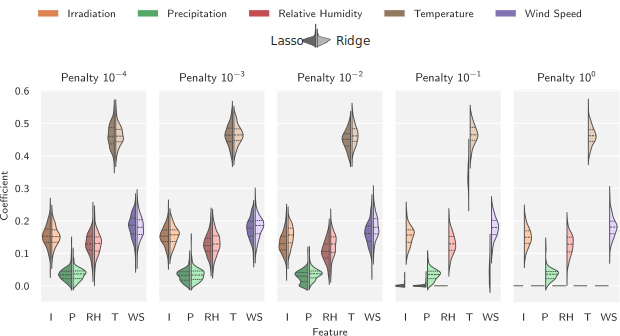
\includegraphics[width=\textwidth]{violins_coefs_ridge-lasso_final}
	\caption{\textbf{Coefficients distributions from Ridge/Lasso feature 	selection} | Bootstrapping for different values of penalties ranging from \num{e-4} to \num{1}; each distribution contains 200 coefficients. Violins are splitted -- the right half corresponds to Ridge fits, the left to Lasso. The three hashed lines in each violins denotes the first interquartile, the median and the third interquartile respectively. In general, Ridge yields slightly higher values, and Lasso shrinks all the coefficients to 0 as applied penalties are in the order of magnitude of $\num{e-1}$ or higher.}
	\label{fig:violins}
\end{figure*}
Insights about the bases of Neural Networks (NNs) are provided in \href{https://github.com/p-perrone/UiO_MachineLearning/blob/main/ml_project2/latex/Perrone_MLProject2.pdf}{report from Project 2}. Particular types of NNs are Recurrent Neural Networks (RNNs). These are a class of NNs specifically designed to model sequential data, by introducing recurrent connections that allow information to persist across time steps. This architecture makes RNNs well suited for time series analysis, where temporal dependencies play a fundamental role \parencite{goodfellow_2016, elmanFindingStructureTime1990}. 

However, standard RNNs suffer from vanishing and exploding gradient problems, which limit their ability to learn long-term dependencies. Long Short-Term Memory (LSTM) networks address these issues through gated memory cells that regulate the flow of information, enabling stable learning over longer sequences and improving performance in many geoscientific and meteorological forecasting applications \parencite{hochreiters.LongShortTermMemory1997,hewageLongshortTermMemory2019}.

	\paragraph{LSTM functioning}
At each time step $t$ the LSTM maintains two states:
\begin{itemize}
	\item a hidden state $\mathbf{h}\curr$;
	\item a cell state $\mathbf{C}\curr$
\end{itemize}
Given the input vector $\mathbf{x}\curr \in \mathbb{R}^n$, the previous hidden state $\mathbf{h}\prev$, and the previous cell state $\mathbf{C}\prev$, the LSTM update equations are defined as follows \parencite{raschkaPythonMachineLearning2017, goodfellow_2016}.

\paragraph{Forget gate}
The forget gate controls how much information from the previous cell state is retained:
\begin{equation}
	\mathbf{f}\curr = \sigma(\bs{W}_{\mathrm{fx}}\mathbf{x}\curr + \bs{W}_{\mathrm{fh}}\mathbf{h}\prev + \mathbf{b}_\mathrm f)
\end{equation}
Here, $\sigma(\cdot)$ denotes the sigmoid activation function. An overview of different activation functions is provided in \pjtwo. $\bs{W}_{\mathrm{fx}}$, $\bs{W}_{\mathrm{fh}}$ and $\mathbf{b}_{\mathrm{f}}$ are the different sets of weights and biases for this gate (the same will be for the following ones). 

\paragraph{Input gate}
The input gate determines how much new information is written to the cell state. It consists of both a sigmoid function, which defines what percentage of the input will be stored in the long-term memory cell, and the $\tanh$ function, which determines what is the full memory that can be stored in the long term memory. These results can be calculated and multiplied together, their sum it is added to the cell state or stored in the long-term memory, denoted as $\mathbf{g}\curr\,\oplus\, \mathbf{i}\curr$:
\begin{align}
	\mathbf{i}\curr &= \sigma(\bs{W}_{\mathrm{ix}}\mathbf{x}\curr + \bs{W}_{\mathrm{ih}}\mathbf{h}\prev + \mathbf{b}_\mathrm{i}) \\
	\mathbf{g}\curr &= \tanh \left(\bs{W}_{\mathrm{gx}}\mathbf{x}\curr + \bs{W}_{\mathrm{gh}}\mathbf{h}\prev + \mathbf{b}_\mathrm{g}\right)
\end{align}

\paragraph{Candidate cell state}
A candidate update for the cell state is computed as:
\begin{equation}
	\tilde{\mathbf{C}}\curr = \tanh\left( \bs{W}_\mathrm{C} \mathbf{x}\curr + \mathbf{b}_\mathrm{C} \mathbf{h}\prev + \mathbf{b}_\mathrm{C} \right).
\end{equation}

\paragraph{Cell state update}
The new cell state combines retained memory and newly acquired information:
\begin{equation}
	\mathbf{C}\curr = \mathbf{f}\curr \odot \mathbf{C}\prev + \mathbf{i}\curr \odot \tilde{\mathbf{C}}\prev
\end{equation}
where $\odot$ denotes element-wise multiplication.

\paragraph{Output gate}
The output gate regulates how much of the cell state is exposed to the hidden state:
\begin{equation}
	\mathbf{o}\curr = \sigma\left( \bs{W}_\mathrm{ox} \mathbf{x}\curr + \bs{W}_\mathrm{ox} \mathbf{h}\prev + \mathbf{b}_\mathrm{o} \right).
\end{equation}

\paragraph{Hidden state update}
The hidden state is finally updated as:
\begin{equation}
	\mathbf{h}\curr = \mathbf{o}\curr \odot \tanh\left( \mathbf{C}\curr \right).
\end{equation}

\paragraph{Vectorized formulation}
For computational efficiency, the gate computations are often implemented in a single matrix operation:
\begin{equation}
	\begin{bmatrix}
		\mathbf{f}\curr \\
		\mathbf{i}\curr \\
		\tilde{\mathbf{C}}\curr \\
		\mathbf{o}\curr
	\end{bmatrix}
	=
	\begin{bmatrix}
		\sigma \\
		\sigma \\
		\tanh \\
		\sigma
	\end{bmatrix}
	\left(
	\bs{W}
	\begin{bmatrix}
		\mathbf{x}\curr \\
		\mathbf{h}\prev
	\end{bmatrix}
	+
	\mathbf{b}
	\right).
\end{equation}

A schematic view of LSTM functioning is shown in Figure \ref{fig:lstm},

\subsubsection{Evaluation of the model: Root Mean Squared Error (RMSE)}
The performance of the model is evaluated by computing the discrepancy between forecasted and observed values of the target variable, after inverse scaling has restored physical units. Given observed values $\mathbf{y} = (y_1,\dots,y_n)$ and corresponding forecasts $\tilde{\mathbf{y}} = (\tilde{y}_1,\dots,\tilde{\tilde{y}}_n)$, the Root Mean Squared Error \parencite{aaaaaaaaaaaaaaaaaaa} is defined as:
\begin{equation}
	\operatorname{RMSE}(\tilde{\mathbf{y}}) 
	= \sqrt{\frac{1}{n}\sum_{i=1}^{n}\left(\tilde{y}_i - y_i\right)^2}.
\end{equation}

For snow depth retrieval, particularly, a further information about model quality is given by the ratio of RMSE to total rime-averaged snowpack thickness, both expressed in \unit{\centi\meter}, \ie the Normalized Root Mean Squared Error \parencite{moriasin.ModelEvaluationGuidelines2007}:
\begin{equation}
	R = \dfrac{\operatorname{RMSE}}{\bar{H}} \times 100 \quad (\%),
\end{equation}
with
\begin{equation}
	\bar{H} = \frac{1}{n}\sum_{i=1}^{n} y_i.
\end{equation}

\subsection{Implementation}

	\subsubsection{Preprocessing}
\begin{figure}[t]
	\centering
	\includegraphics[width=\columnwidth]{heatmap_stability_lasso}
	\caption{\textbf{Sign--stability of Lasso fits over 200 bootstraps as function of penalty} | Values between 0.9 and 1 indicate consistent sign in the same coefficient distribution. In general, this result is achieved for $\alpha \geq e-2$.}
	\label{fig:signstability}
\end{figure}
The data from Pont weather station were loaded in in a Python 3.12 environment and organized in a dataframe using \texttt{glob} and \texttt{pandas} modules \parencite{pandas_docs, python_glob}, with time steps as indexes and variables as columns. This part was performed in two steps, as we decided to include in the analysis wind speed only in a second moment, taking the occasion to enlarge the dataset timespan.
\begin{figure}[t]
	\centering
	\includegraphics[width=\columnwidth]{mse_vs_alpha_lasso}
	\caption{\textbf{MSE from Lasso with different regularizations} | The error between observed and modeled snow depths exponentially increases for $\alpha \geq 1$.}
	\label{fig:mselasso}
\end{figure}
The loaded dataframe contained NaNs. Some rows were entirely NaNs (missing values for every variable) -- we directly excluded these rows from further computations. For single or small gaps, we applied forward and backward filling, that consist in replacing missing values at time step (index) \texttt{t} with the value recorded at \texttt{t-1} or \texttt{t+1}. This gap filling method was confirmed to be one of the most efficient when handling small gaps meteorological data, since it is simple, stable and accurate based on RMSE results \parencite{siabiEffectiveMethodFilling2022}.

Most of the preprocessing was performed using \sk utilities \parencite{scikit-learn-selectfrommodel-diabetes, sklearn_docs}. Column-wise scaling was carried out with \sk \texttt{StandardScaler} class to ensure numerical stability, as previously explained.

Train-test splitting was handled separately and differently for feature selection ad LSTM modeling, hence it is not included in this part of the workflow.

	\subsubsection{Feature selection}
Since snow depth is our focus, feature selection was carried out to investigate which other parameters had the strongest influence on it. 

In the order:
\begin{enumerate}
	\item the dataset was split with \sk \texttt{train\_test\_split} function, setting all the steps before December 2 as training set;
	\item for different values of penalties $\alpha$ ranging from \num{e-5} to 1:
	\subitem -- Ridge ad Lasso fits were computed with bootstrapping (200 bootstraps), resulting in a distribution of coefficients for each meteorological variable;
	\subitem -- the sign-stability and MSE were computed from these distributions;
	\item the penalty value that yielded the best combination of MSE and sign--stability was used to select the essential features for snow depth forecasting, again bootstrapping Lasso fit over 400 iterations and filtering with the threshold criterion (Equation \eqref{eq:tsc}).
\end{enumerate}

This tuning workflow was carried out by creating custom functions, one for the metrics (\texttt{stability\_mse()}) and one for the actual feature selection (\texttt{feature\_selection()}). Note that, for feature selection, the MSE is computed using snow depth values modeled over the same time period in which the meteorological observations are available; the forecasting task is addressed separately in the following section.
\begin{figure*}[h]
	\centering
	\includegraphics[width=\textwidth]{hm_activations_epochs_final}
	\caption{\textbf{MSE of LSTM forecasts for different activation functions and number of epochs} | The bars refer to MSE values expressed in squared predictor unit. Values above 50 are displayed in light gray. The best (minimum) MSE is highlighted in red dashed line.}
	\label{fig:actepochs}
\end{figure*}
	\subsubsection{Forecasting}
Splitting of the dataset in a test and training sets was done manually by setting a split time (December 2 at 00:00).

The original hourly meteorological time series were first transformed into supervised learning samples through a sliding-window sequencing approach. The \texttt{create\_sequence} custom function transforms raw time series data of shape \texttt{(n, p)}, with \texttt{n} the number of samples and \texttt{p} the number of features, into input-output pairs suitable for sequence models such as LSTMs. For a given sequence length, in our case typically 48 hours, the function extracts overlapping sequences of past observations as model inputs, and for a forecast horizon (24 hours), it extracts the corresponding future values of the target variable as outputs. If the input is a \texttt{pandas} DataFrame, the specified feature columns are stacked alongside the target column, with the target always placed last to simplify slicing. The function iterates over the dataset, generating arrays of shape \texttt{(n, sequence\_length, p)} and Y of shape (n, forecast\_horizon). 

This setup allows the LSTM to learn temporal dependencies from past features to predict multiple future steps of the target variable, effectively framing time series forecasting as a supervised learning problem.

The implementation of LSTM was straight-forward with \tf (\url{https://www.tensorflow.org/}), a machine learning-oriented Python ecosystem. Its library \texttt{keras} is particularly suitable for sequential models such as RNNs (\url{https://keras.io/}). We structured our code using \texttt{keras.models.Sequential()} as base model, and \texttt{keras.layers.LSTM()} and \texttt{keras.layers.Dense()} as layers. The workflow we followed to build this model is largely inspired to this \href{https://www.tensorflow.org/tutorials/structured_data/time_series}{notebbok} \parencite{tensorflow_timeseries, tensorflow_sequential}. A typical implementation in Python would be the following;
\begin{python}
	model = Sequential([
		LSTM(units=32, 
			input_shape=(timesteps, n_features)
			),
		Dense(horizon)
		])
	model.compile(
			optimizer='adam', 
			loss='mse',
	)
	model.fit(X_train, y_train, 
			epochs=50, 
			batch_size=16,)
\end{python}
The LSTM layer receives input sequences of shape 
\texttt{(timesteps, n\_features)} and learns temporal dependencies across the input window, compressing the sequence information into a latent representation of size units. The subsequent Dense layer maps this representation to the forecast horizon, producing a multi-step prediction of the target variable. The model is trained using the Adam optimizer, since it is the most efficient according to \pjtwo, and by minimizing the MSE loss. Training is performed over multiple epochs with mini-batches, allowing the network to iteratively adjust its parameters to capture the temporal dynamics of the data.

We organized forecasting by modeling both snow depth and temperature in the future 24 hours (\emph{i.e.}, \texttt{horizon}). In fact, even is our focus is primarily snow pack, temperature patterns have a more 'predictable' behavior as more influenced from diurnal cycles of solar radiation; it can therefore be a reference benchmark for evaluating the network, whereas snow pack is more experimentally complicated to forecast \parencite{dewallePrinciplesSnowHydrology2008, lehningPhysicalSNOWPACKModel2002, blandiniLearningFilterSnow2025}. Since features were not selected for temperature, this was fitted using all the variables. Snow depth was fitted both with the full features set (snow depth itself, irradiation, precipitation, relative humidity, wind speed and temperature) \emph{and} with the features previously selected only. We end up with we three sets to model, in the end.

Model tuning was carried out by gradually seeking MSE minima in simulation results obtained with different ranges of selected hyperparameters. For the three target sets, we evaluated MSEs between the observed and forecasted values by exploring the dependence of fit quality on:
\begin{enumerate}[(1)]
	\item the choice of activation function for the \texttt{LSTM} layer and the number of epochs;
	\item the number of units in the \texttt{LSTM} layer and the use of a bias initializer, employing the optimal activation and epochs found in (1).
\end{enumerate}

The bias initializer can be passed as an argument to the \texttt{Dense} layer, for instance by using the mean of the last 12 hours of observations in the pre-forecasting period. Potentially, this may improve the fit by biasing the forecast toward a more realistic value than the default random bias.

Finally, we performed a forecast with the optimal combination of the four hyperparameters (activation function, epochs, units, and bias initializer) and computed RMSE and NRMSE between the modeled and observed series.

\subsection{Use of Artificial Intelligence}
ChatGPT service from Open AI was used both in browser version and VSCode AI Chat. It was mainly employed to fix, debug or improve custom functions and fairly complex plots (such as Figure \ref{fig:violins}). Whether this tool was used, a comment line in the code specifies it, both in GitHub-available \texttt{functions.py} file and in the analysis notebook. The employed online chat can be visited at \url{CHATGPTCHAT}. For bibliography, Google Scholar Labs provided a fast and efficient way to find studies comparable to this work.

\begin{figure*}[h]
	\centering
	\includegraphics[width=0.8\textwidth]{mse_bins_final}
	\caption{\textbf{MSE of LSTM forecasts for different units amount and with/without bias initialization} | For each units range, left and pastel bins refer to random bias initialization (\texttt{None}); right, saturated bins refer to bias initialization using the mean of last 12 hours of training series (before the start of forecasting period). $y$-axis is truncated at MSE = 60, longer bins are displayed with an upward arrow. Optimal combinations of activation function and epochs were set after the first tuning phase (Figure \ref{fig:actepochs}).}
	\label{fig:bins}
\end{figure*}

\section{Results and discussions}
\begin{table}
	\small
	\centering
	\caption{Lasso coefficients for snow depth prediction.}
	\begin{tabular}{
			p{1.8cm}
			S[scientific-notation = true]
			S[scientific-notation = true]
		}
		\toprule
		Predictor & {Coef.} & {Std. error} \\
		(unit)    & {(cm\,unit$^{-1}$)} & {(cm\,unit$^{-1}$)} \\
		\midrule
		Irradiation (W\,m$^{-2}$)     & 0        & 5.9e-3  \\
		Precipitation (mm\,h$^{-1}$)  & 0        & 7.0e-3  \\
		Relative humidity (\%)         & 0        & 1.1e-3  \\
		Wind speed (m\,s$^{-1}$)      & 4.2e-2   & 3.0e-2 \\
		Temperature (°C)              & -3.3e-1  & 2.7e-2 \\
		\bottomrule
	\end{tabular}
	\label{tab:fscoefs}
\end{table}
\subsection{Feature selection}
The results of the bootstrapped Ridge and Lasso fits are shown in Figure \ref{fig:violins}. Ridge generally yields slightly larger coefficient values than Lasso and, as expected, does not shrink any of them to zero, whereas Lasso drives several coefficients to zero for penalties $\alpha \geq \num{e-1}$. Temperature exhibits by far the strongest effect, with mean coefficients 3–10 times larger than those of the other predictors in both methods. This outcome is consistent with previous studies that relied solely on temperature to estimate snowpack or ice dynamics, for example Degree-day approaches used to model melt rates \parencite{hockDistributedTemperatureindexIce1999, braithwaitePositiveDegreedayFactors1995, Hachem2009:modis_permafrost_mapping}.
Sign–stability and MSEs computed from these fits suggest selecting features using $\alpha = 0.1$, as it represents an appropriate tradeoff between penalization and accuracy, with a sign–stability of 0.91 (Figure \ref{fig:signstability}) and an MSE of 0.65 (Figure \ref{fig:mselasso}). Hence, with $\alpha = 0.1$, Lasso regression yields the coefficients in Table \ref{tab:fscoefs}, indicating that temperature and wind speed should be selected as the primary predictors. This result is partially consistent with existing literature: temperature remains the major regulator of snowpack evolution. Although wind can be considered an informative predictor, its influence is generally weaker than that of precipitation: correlation coefficients between snow pack thickness and snowfall intensity are usually $\sim2$ times larger than snow depth/wind speed ones. \parencite{durandMeteorologicalEstimationRelevant1993, maSnowDepthVariability2023, dadicWindInfluenceSnow2010}. The relatively small weight assigned to irradiation is likely related to the topographic context of the Pont weather station: the narrow, flat valley bottom exhibits limited contrasts in daytime irradiation, and the amount of solar radiation received at the surface in winter is reduced.

\subsection{LSTM forecasting}
The results of LSTM model tuning are showed in Figures \ref{fig:actepochs} and \ref{fig:bins}. In general, all the MSEs are fairly high, always included in the range 3.4 -- \num{e3}. This is a first indicator of model incapacity to correctly reproduce patterns in the future, especially when a little amount of predictor is set. We would rather expect MSE below 1, to potentially compare our model architecture with the ones of similar, but more effective studies, such as \cite{blandiniLearningFilterSnow2025, wangExploringPotentialLong2022}. In fact, trying to forecast snow depth using temperature and wind speed solely leads to poor quality predictions. When all the predictors are included in the model, the 24 hours-forecasted snow depth approximate the finally observed values much better. LSTM still yields best results with temperature forecasts, with the lowest recorded MSEs, both for the first tuning phase (activation function -- epochs dependency) and the second (LSTM units -- bias initializer dependency).

From Figure \ref{fig:actepochs}, we can assess the optimal combination of activation function and epochs range: (Sigmoid, 150 epochs) for temperature prediction, (ReLu, 75 epochs) for snow depth with all predictors, (Linear, 125) for snow depth with selected features. Since trends in MSEs are barely visible (\ie, no strong dependencies on epochs range), it also is difficult to assess whether these combinations are effective or just random effects-related. Still, we set them as constant hyperparameters for the following part.

Figure \ref{fig:bins} is 

\printbibliography[heading=bibintoc]

\end{document}